\documentclass{ximera}

\author{Bart Snapp}

\usepackage[T1]{fontenc}
\usepackage{stix2}
\usepackage{gillius}
\usepackage{resizegather}
%\usepackage{rsfso} fancy cal
\DeclareMathAlphabet{\mathcal}{OMS}{cmsy}{m}{n} %less fancy cal


\usepackage{multicol}


\usepackage{tikz-cd}
\usepackage{tkz-euclide} %% compass
\usetkzobj{all}  %% tkzCompass
\tikzset{>=stealth}
\tikzcdset{arrow style=tikz}
\usetikzlibrary{math} %% for assigning variables
%\usetikzlibrary{fadings}

\usepackage{colortbl,boldline,makecell} %% group tables


\usepackage[sans]{dsfont}

\usepackage{stmaryrd,pifont}

\graphicspath{
  {./}
  {fields/}
  }     



\let\oldbibliography\thebibliography%% to compact bib
\renewcommand{\thebibliography}[1]{%
  \oldbibliography{#1}%
  \setlength{\itemsep}{0pt}%
}
\renewcommand\refname{} %% no name needed!


\DefineVerbatimEnvironment{macaulay2}{Verbatim}{numbers=left,frame=lines,label=Macaulay2,labelposition=topline}

\DefineVerbatimEnvironment{gap}{Verbatim}{numbers=left,frame=lines,label=GAP,labelposition=topline}

%%% This next bit of code defines all our theorem environments
\makeatletter
\let\c@theorem\relax
\let\c@corollary\relax
%\let\c@example\relax
\makeatother

\let\definition\relax
\let\enddefinition\relax

\let\theorem\relax
\let\endtheorem\relax

\let\proposition\relax
\let\endproposition\relax

\let\exercise\relax
\let\endexercise\relax

\let\question\relax
\let\endquestion\relax

\let\remark\relax
\let\endremark\relax

\let\corollary\relax
\let\endcorollary\relax


\let\example\relax
\let\endexample\relax

\let\warning\relax
\let\endwarning\relax

\let\lemma\relax
\let\endlemma\relax


\let\algorithm\relax
\let\endalgorithm\relax
\usepackage{algpseudocode}

\newtheoremstyle{SlantTheorem}{\topsep}{\topsep}%%% space between body and thm
		{\slshape}                      %%% Thm body font
		{}                              %%% Indent amount (empty = no indent)
		{\bfseries\sffamily}            %%% Thm head font
		{}                              %%% Punctuation after thm head
		{3ex}                           %%% Space after thm head
		{\thmname{#1}\thmnumber{ #2}\thmnote{ \bfseries(#3)}}%%% Thm head spec
\theoremstyle{SlantTheorem}
\newtheorem{theorem}{Theorem}
%\newtheorem{definition}[theorem]{Definition}
%\newtheorem{proposition}[theorem]{Proposition}
%% \newtheorem*{dfnn}{Definition}
%% \newtheorem{ques}{Question}[theorem]
%% \newtheorem*{war}{WARNING}
%% \newtheorem*{cor}{Corollary}
%% \newtheorem*{eg}{Example}
\newtheorem*{remark}{Remark}
\newtheorem*{touchstone}{Touchstone}
\newtheorem{corollary}{Corollary}[theorem]
\newtheorem*{warning}{WARNING}
\newtheorem{example}[corollary]{Example}
\newtheorem{lemma}[theorem]{Lemma}




\newtheoremstyle{Definition}{\topsep}{\topsep}%%% space between body and thm
		{}                              %%% Thm body font
		{}                              %%% Indent amount (empty = no indent)
		{\bfseries\sffamily}            %%% Thm head font
		{}                              %%% Punctuation after thm head
		{3ex}                           %%% Space after thm head
		{\thmname{#1}\thmnumber{ #2}\thmnote{ \bfseries(#3)}}%%% Thm head spec
\theoremstyle{Definition}
\newtheorem{definition}[theorem]{Definition}



\let\algorithm\relax
\let\endalgorithm\relax
\newtheoremstyle{Alg}{\topsep}{\topsep}%%% space between body and thm
		{}                              %%% Thm body font
		{}                              %%% Indent amount (empty = no indent)
		{\bfseries\sffamily}            %%% Thm head font
		{}                              %%% Punctuation after thm head
		{3ex}                           %%% Space after thm head
		{\thmname{#1}\thmnumber{ #2}\thmnote{ \bfseries(#3)}}%%% Thm head spec
\theoremstyle{Alg}
\newtheorem*{algorithm}{Algorithm}
\newtheorem*{construction}{Construction}




\newtheoremstyle{Exercise}{\topsep}{\topsep} %%% space between body and thm
		{}                           %%% Thm body font
		{}                           %%% Indent amount (empty = no indent)
		{\bfseries\sffamily}         %%% Thm head font
		{)}                          %%% Punctuation after thm head
		{ }                          %%% Space after thm head
		{\thmnumber{#2}\thmnote{ \bfseries(#3)}}%%% Thm head spec
\theoremstyle{Exercise}
\newtheorem{exercise}[corollary]{}%[theorem]

%% \newtheoremstyle{Question}{\topsep}{\topsep} %%% space between body and thm
%% 		{\bfseries}                  %%% Thm body font
%% 		{3ex}                        %%% Indent amount (empty = no indent)
%% 		{}                           %%% Thm head font
%% 		{}                           %%% Punctuation after thm head
%% 		{}                           %%% Space after thm head
%% 		{\thmnumber{#2}\thmnote{ \bfseries(#3)}}%%% Thm head spec
\newtheoremstyle{Question}{3em}{3em} %%% space between body and thm
		{\large\bfseries}                           %%% Thm body font
		{}                           %%% Indent amount (empty = no indent)
		{}                         %%% Thm head font
		{}                          %%% Punctuation after thm head
		{0em}                          %%% Space after thm head
		{}%%% Thm head spec
\theoremstyle{Question}
\newtheorem*{question}{}






\renewcommand{\tilde}{\widetilde}
\renewcommand{\bar}{\overline}
\renewcommand{\hat}{\widehat}
\newcommand{\N}{\mathbb N}
\newcommand{\Z}{\mathbb Z}
\newcommand{\R}{\mathbb R}
\newcommand{\Q}{\mathbb Q}
\newcommand{\C}{\mathbb C}
\newcommand{\V}{\mathbb V}
\newcommand{\I}{\mathbb I}
\newcommand{\A}{\mathbb A}
\renewcommand{\o}{\mathbf o}
\newcommand{\iso}{\simeq}
\newcommand{\ph}{\varphi}
\newcommand{\Cf}{\mathcal{C}}
\newcommand{\IZ}{\mathrm{Int}(\Z)}
\newcommand{\dsum}{\oplus}
\newcommand{\directsum}{\bigoplus}
\newcommand{\union}{\bigcup}
\newcommand{\subgp}{\leq}
\newcommand{\normal}{\trianglelefteq}
\renewcommand{\i}{\mathfrak}
\renewcommand{\a}{\mathfrak{a}}
\renewcommand{\b}{\mathfrak{b}}
\newcommand{\m}{\mathfrak{m}}
\newcommand{\p}{\mathfrak{p}}
\newcommand{\q}{\mathfrak{q}}
\newcommand{\dfn}[1]{\textbf{#1}\index{#1}}
\let\hom\relax
\DeclareMathOperator{\mat}{Mat}
\DeclareMathOperator{\ann}{Ann}
\DeclareMathOperator{\h}{ht}
\DeclareMathOperator{\tr}{tr}
\DeclareMathOperator{\hom}{Hom}
\DeclareMathOperator{\Span}{Span}
\DeclareMathOperator{\spec}{Spec}
\DeclareMathOperator{\maxspec}{MaxSpec}
\DeclareMathOperator{\aut}{Aut}
\DeclareMathOperator{\ass}{Ass}
\DeclareMathOperator{\lcm}{lcm}
\DeclareMathOperator{\ff}{Frac}
\DeclareMathOperator{\im}{Im}
\DeclareMathOperator{\syz}{Syz}
\DeclareMathOperator{\gr}{Gr}
\DeclareMathOperator{\multideg}{multideg}
\renewcommand{\ker}{\mathop{\mathrm{Ker}}\nolimits}
\newcommand{\coker}{\mathop{\mathrm{Coker}}\nolimits}
\newcommand{\lps}{[\hspace{-0.25ex}[}
\newcommand{\rps}{]\hspace{-0.25ex}]}
\newcommand{\into}{\hookrightarrow}
\newcommand{\onto}{\twoheadrightarrow}
\newcommand{\tensor}{\otimes}
\newcommand{\x}{\mathbf{x}}
\newcommand{\X}{\mathbf X}
\newcommand{\Y}{\mathbf Y}
\renewcommand{\k}{\boldsymbol{\kappa}}
\renewcommand{\emptyset}{\varnothing}
\renewcommand{\qedsymbol}{$\blacksquare$}
\renewcommand{\l}{\ell}
\newcommand{\1}{\mathds{1}}
\newcommand{\lto}{\mathop{\longrightarrow\,}\limits}
\newcommand{\rad}{\sqrt}
\newcommand{\hf}{H}
\newcommand{\hs}{H\!S}
\newcommand{\hp}{H\!P}
\renewcommand{\vec}{\mathbf}
\let\temp\phi
\let\phi\varphi
\let\eulerphi\temp


\renewcommand{\epsilon}{\varepsilon}
\renewcommand{\subset}{\subseteq}
\renewcommand{\supset}{\supseteq}
\newcommand{\macaulay}{\normalfont\textsl{Macaulay2}}
\newcommand{\GAP}{\normalfont\textsf{GAP}}
\newcommand{\invlim}{\varprojlim}
\renewcommand{\le}{\leqslant}
\renewcommand{\ge}{\geqslant}
\newcommand{\valpha}{{\boldsymbol\alpha}}
\newcommand{\vbeta}{{\boldsymbol\beta}}
\newcommand{\vgamma}{{\boldsymbol\gamma}}
\newcommand{\dotp}{\bullet}
\newcommand{\lc}{\normalfont\textsc{lc}}
\newcommand{\lt}{\normalfont\textsc{lt}}
\newcommand{\lm}{\normalfont\textsc{lm}}
\newcommand{\from}{\leftarrow}
\newcommand{\transpose}{\intercal}
\newcommand{\grad}{\boldsymbol\nabla}
\newcommand{\curl}{\boldsymbol{\nabla\times}}
\renewcommand{\d}{\, d}
\newcommand{\<}{\langle}
\renewcommand{\>}{\rangle}

%\renewcommand{\proofname}{Sketch of Proof}


\renewenvironment{proof}[1][Proof]
  {\begin{trivlist}\item[\hskip \labelsep \itshape \bfseries #1{}\hspace{2ex}]\upshape}
{\qed\end{trivlist}}

\newenvironment{sketch}[1][Sketch of Proof]
  {\begin{trivlist}\item[\hskip \labelsep \itshape \bfseries #1{}\hspace{2ex}]\upshape}
{\qed\end{trivlist}}



\makeatletter
\renewcommand\section{\@startsection{paragraph}{10}{\z@}%
                                     {-3.25ex\@plus -1ex \@minus -.2ex}%
                                     {1.5ex \@plus .2ex}%
                                     {\normalfont\large\sffamily\bfseries}}
\renewcommand\subsection{\@startsection{subparagraph}{10}{\z@}%
                                    {3.25ex \@plus1ex \@minus.2ex}%
                                    {-1em}%
                                    {\normalfont\normalsize\sffamily\bfseries}}
\makeatother

%% Fix weird index/bib issue.
\makeatletter
\gdef\ttl@savemark{\sectionmark{}}
\makeatother


\makeatletter
%% no number for refs
\newcommand\frontstyle{%
  \def\activitystyle{activity-chapter}
  \def\maketitle{%
    \addtocounter{titlenumber}{1}%
                    {\flushleft\small\sffamily\bfseries\@pretitle\par\vspace{-1.5em}}%
                    {\flushleft\LARGE\sffamily\bfseries\@title \par }%
                    {\vskip .6em\noindent\textit\theabstract\setcounter{problem}{0}\setcounter{sectiontitlenumber}{0}}%
                    \par\vspace{2em}
                    \phantomsection\addcontentsline{toc}{section}{\textbf{\@title}}%
                  }}
\makeatother



\NewEnviron{annotate}{\vspace{-.3cm}\small \itshape \BODY \vspace{.3cm}}


%%%% TIKZ STUFF

%% N-GON code
\tikzset{
    pics/tikzngon/.style={
        code={
        \tikzmath{\xx = #1;\rr=1.7;}
        \draw[ultra thick,rounded corners=.05mm] ({\rr*sin(0*360/\xx)},{\rr*cos(0*360/\xx)})
        \foreach \x in {-1,0,...,\xx}
        {
        -- ({\rr*sin(\x*360/\xx)},{\rr*cos(\x*360/\xx)})
        }
           -- cycle;
  }}}

%% N-GON code (even)
\tikzset{
    pics/tikzegon/.style={
        code={
        \tikzmath{\xx = #1;\rr=1.7;}
        \draw[ultra thick,rounded corners=.05mm] ({\rr*sin(0*360/\xx+180/\xx)},{\rr*cos(0*360/\xx+180/\xx)})
        \foreach \x in {-1,0,...,\xx}
           {
           -- ({\rr*sin(\x*360/\xx+180/\xx)},{\rr*cos(\x*360/\xx+180/\xx)}) 
           }
           -- cycle;
  }}}




%% N-CLOCK code
\tikzset{
    pics/tikznclock/.style={
        code={
        \tikzmath{\xx = #1;\rr=1.7;\dd=.4;}
        \foreach \x in {1,...,\xx}
        \pgfmathtruncatemacro{\xy}{\x-1}
           {
             \node[circle,fill=black,inner sep=0pt, minimum size=13pt,text=white]
             at ({(\rr-\dd)*sin((\x-1)*360/(\xx)},{(\rr-\dd)*cos((\x-1)*360/\xx}) {\normalfont\bfseries\sffamily\small {\xy}};
           }
  \draw[thick] (0,0) circle (\rr);
  }}}



%% barcode from
%% https://tex.stackexchange.com/questions/6895/is-there-a-good-latex-package-for-generating-barcodes
%% NOT CURRENTLY USED!


\def\barcode#1#2#3#4#5#6#7{\begingroup%
  \dimen0=0.1em
  \def\stack##1##2{\oalign{##1\cr\hidewidth##2\hidewidth}}%
  \def\0##1{\kern##1\dimen0}%
  \def\1##1{\vrule height10ex width##1\dimen0}%
  \def\L##1{\ifcase##1\bc3211##1\or\bc2221##1\or\bc2122##1\or\bc1411##1%
    \or\bc1132##1\or\bc1231##1\or\bc1114##1\or\bc1312##1\or\bc1213##1%
    \or\bc3112##1\fi}%
  \def\R##1{\bgroup\let\next\1\let\1\0\let\0\next\L##1\egroup}%
  \def\G##1{\bgroup\let\bc\bcg\L##1\egroup}% reverse
  \def\bc##1##2##3##4##5{\stack{\0##1\1##2\0##3\1##4}##5}%
  \def\bcg##1##2##3##4##5{\stack{\0##4\1##3\0##2\1##1}##5}%
  \def\bcR##1##2##3##4##5##6{\R##1\R##2\R##3\R##4\R##5\R##6\11\01\11\09%
    \endgroup}%
  \stack{\09}#1\11\01\11\L#2%
  \ifcase#1\L#3\L#4\L#5\L#6\L#7\or\L#3\G#4\L#5\G#6\G#7%
    \or\L#3\G#4\G#5\L#6\G#7\or\L#3\G#4\G#5\G#6\L#7%
    \or\G#3\L#4\L#5\G#6\G#7\or\G#3\G#4\L#5\L#6\G#7%
    \or\G#3\G#4\G#5\L#6\L#7\or\G#3\L#4\G#5\L#6\G#7%
    \or\G#3\L#4\G#5\G#6\L#7\or\G#3\G#4\L#5\G#6\L#7%
  \fi\01\11\01\11\01\bcR}


\title{Algebra is geometry}

\begin{document}
\begin{abstract}
  We analyze which numbers can be constructed via compass and
  straightedge.
\end{abstract}
\maketitle


Now we will combine two areas of mathematics: Algebra and
geometry. Gauss was the first to do this, and we will be inspired by
his work.

\section{Geometry}

Around 300 BCE, Euclid, wrote \textit{The Elements.} This is a book
that is widely accepted to be the first ``axiomatic'' approach to
mathematics. It was used as a text for higher-education for around
2000 years, and it is surely the most successful textbook ever
written. In this work, Euclid states five so-called postulates:
\begin{enumerate}
\item[(1)] To draw a straight line from any point to any point.
\item[(2)] To produce a finite straight line continuously in a straight line.
\item[(3)] To describe a circle with any center and radius.
\item[(4)] That all right angles equal one another.
\item[(5)] That, if a straight line falling on two straight lines makes the
  interior angles on the same side less than two right angles, the two
  straight lines, if produced indefinitely, meet on that side on which
  are the angles less than the two right angles.
\end{enumerate}
Readers throughout time have interpreted these statements as statements
concerning what is allowed when working with geometry.

Postulates (1) is typically interpreted to mean that, ``if you want to
draw a line, you must be connecting two points.'' \textbf{This is exactly what
you can draw with a straightedge.}


Postulate (2) is interpreted to mean that, ``if you have a central
point, and a point on the circle, then you can draw the circle.''
\textbf{This is exactly what you can draw with a compass.}

Compass and straightedge constructions have lost some of their
practicality with the advent of computer-aided-design. However, it is
worth pointing out some facts.

\paragraph{Compass and straightedge constructions are \textbf{independent of units}.} 
Whether you are working in centimeters or miles, compass and
straightedge constructions work just as well. By not being locked to
set of units, the constructions given by a compass and straightedge
have certain generality that is appreciated even today. For example,
this allowed violin makers of the 1700's to construct shapes for
violins that could be scaled for size of the musician.


\paragraph{Compass and straightedge constructions are \textbf{theoretically correct}.} 
In mathematics, a correct method to solve a problem is more valuable
than a correct solution. In this sense, the compass and straightedge
are ideal tools for the mathematician. Easy enough to use that the
rough drawings that they produce can be somewhat relied upon, yet
simple enough that the tools themselves can be described
theoretically. Hence it is usually not too difficult to connect a
given construction to a formal proof showing that the construction is
correct.


\paragraph{Combined, the compass and straightedge seem like \textbf{powerful tools}.} 
No tool is useful unless it can solve a lot of problems. Without a
doubt, the compass and straightedge combined form a powerful
tool. Using a compass and straightedge, we are able to solve many
problems exactly. Of the problems that we cannot solve exactly, we can
always produce an approximate solution.


We'll start by giving the rules of compass and straightedge
constructions:

\subsubsection{Rules for Compass and Straightedge Constructions}
\begin{enumerate}
\item You may only use a compass and straightedge.
\item You must have two points to draw a line.
\item You must have a point and a line segment to draw a circle. The
  point is the center and the line segment gives the radius.
\item Points can only be placed in two ways:
\begin{enumerate}
\item As the intersection of lines and/or circles.
\item As a \textbf{free point}\index{free point}, meaning the location
  of the point is not important for the final outcome of the
  construction.
\end{enumerate}
\end{enumerate}



\subsection{Basic constructions}
Our first construction is also Euclid's first construction:

\begin{construction}[Equilateral triangle]\index{compass and straightedge!equilateral triangle} We wish to construct an equilateral triangle given the length of one 
side.
\begin{enumerate} 
\item Open your compass to the width of the line segment.
\item Draw two circles, one with the center being each end point 
of the line segment.
\item The two circles intersect at two points.  Choose one and 
connect it to both of the line segment's endpoints.
\end{enumerate}
\[
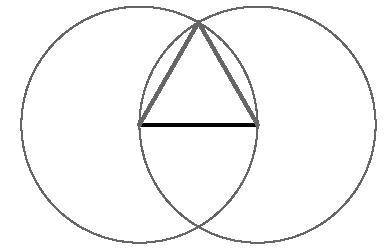
\includegraphics[scale=0.9]{eqtri.pdf}
\]
\end{construction}

Euclid's second construction will also be our second construction:

\begin{construction}[Transferring a segment]\index{compass and straightedge!transferring a segment}
Given a segment, we wish to move it so that it starts on a given
point, on a given line.
\begin{enumerate}        
\item Draw a line through the point in question.
\item Open your compass to the length of the line segment and draw a circle with the given point as its center.
\item The line segment consisting of the given point and the intersection of the circle and the line 
is the transferred segment.
\end{enumerate}
\end{construction}



If you read \textit{The elements}, you'll see that Euclid's construction is
much more complicated than ours.   Apparently, Euclid felt the need to
justify the ability to move a distance. Many sources say that Euclid
used what is called a \index{compass!collapsing}\index{collapsing
compass}\textit{collapsing compass}, that is a compass that collapsed
when it was picked up. However, I do not believe that such an
invention ever existed. Rather this is something that lives in the
conservative geometer's head.


Regardless of whether the difficulty of transferring distances was theoretical
or physical, we need not worry when we do it.  In fact, Euclid's
proof of the above theorem proves that our modern way of using the
compass to transfer distances is equivalent to using the so-called
collapsing compass.





\begin{construction}[Bisecting a segment]\index{compass and straightedge!bisecting a segment} 
Given a segment, we wish to cut it in half.
\begin{enumerate}
\item Open your compass to the width of the segment.
\item Draw two circles, one with the center being at each end point 
of the line segment.
\item The circles intersect at two points.  Draw a line through 
these two points.
\item The new line bisects the original line segment.
\end{enumerate}
\[
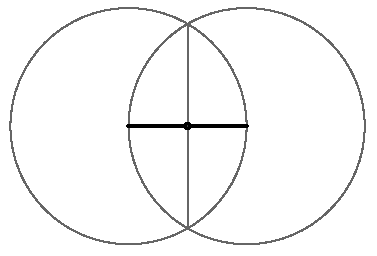
\includegraphics[scale=0.9]{bisectseg.pdf}
\]
\end{construction}

\begin{construction}[Perpendicular to a line through a point]\index{compass and straightedge!perpendicular to a line through a point}  
Given a point and a line, we wish to construct a line perpendicular to
the original line that passes through the given point.
\begin{enumerate}
\item Draw a circle centered at the point large enough  
       to intersect the line in two distinct points.
\item Bisect the line segment. The line used to do this 
       will be the desired line.
\end{enumerate}
\[
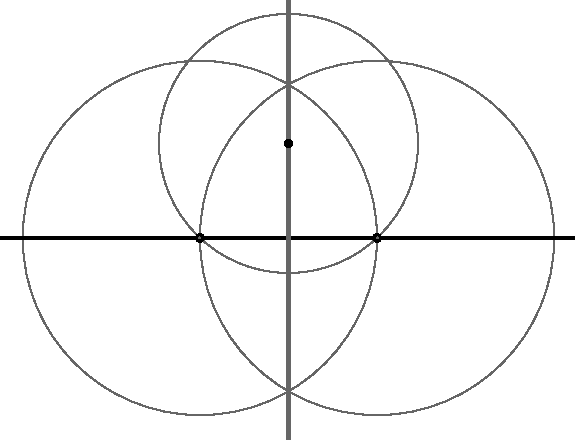
\includegraphics[scale=0.8]{perpfrompoint.pdf}
\]
\end{construction}





\begin{construction}[Bisecting an angle]\index{compass and straightedge!bisecting an angle} 
We wish to divide an angle in half.
\begin{enumerate}
\item Draw a circle with its center being the vertex of the 
angle.
\item Draw a line segment where the circle intersects the lines.
\item Bisect the new line segment.  The bisector will bisect the angle.
\end{enumerate}
\[
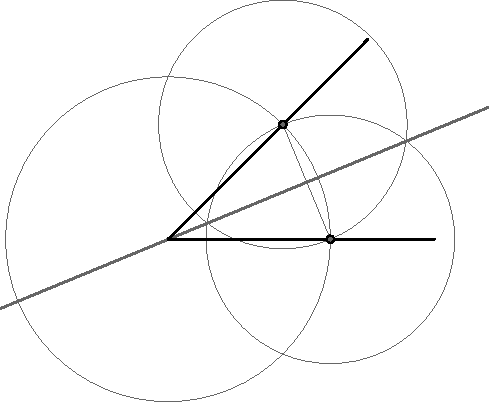
\includegraphics{bisectangle.pdf}
\]
\end{construction}


We now come to a very important construction:

\begin{construction}[Copying an angle]\index{compass and straightedge!copying an angle} 
Given a point on a line and some angle, we wish to copy the 
given angle so that the new angle has the point as its 
vertex and the line as one of its edges.
\begin{enumerate}
\item Open the compass to a fixed width and make a circle 
centered at the vertex of the angle.
\item Make a circle of the same radius on the line with the point.
\item Open the compass so that one end touches the $1$st circle 
where it hits an edge of the original angle, with the other end of the compass extended to where the $1$st circle hits the other edge of the original angle.
\item Draw a circle with the radius found above with its center 
where the second circle hits the line.
\item Connect the point to where the circles meet. This is the other leg of the angle we are constructing.
\end{enumerate}
\[
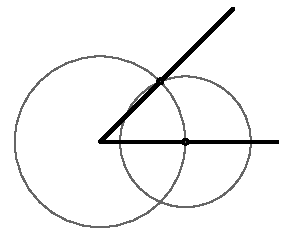
\includegraphics{copyangle.pdf}
\]
\end{construction}



\begin{construction}[Parallel to a line through a point]\index{compass and straightedge!parallel to a line through a point} 
 Given a line and a point, we wish to construct another line parallel
 to the first that passes through the given point.
\begin{enumerate}
\item Draw a circle around the given point that passes through the given line at two points.
\item We now have an isosceles triangle, duplicate this triangle.
\item Connect the top vertexes of the triangles and we get a parallel line.
\end{enumerate}
\vspace{1cm}
\[
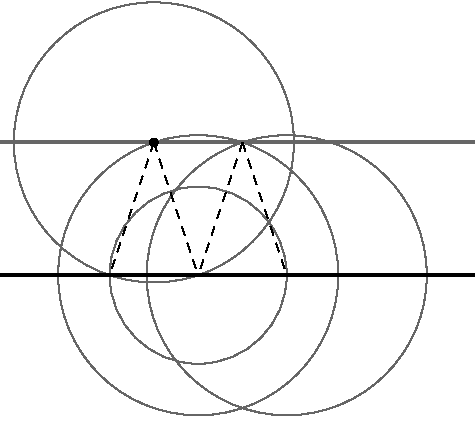
\includegraphics[scale=0.9]{parallel.pdf}
\]
\end{construction}



\section{Geometry and numbers}

In this section, we'll use compass and straightedge to construct $\Z$,
$\Q$, $\Q(i)$, and more.  First we'll construct $\Z$. Start by making
some point the \textbf{origin}:
\[
\begin{tikzpicture}
  \tkzDefPoint(0,0){0}
  \tkzDrawPoint[fill=black](0)
  \tkzLabelPoints[below](0)
\end{tikzpicture}
\]
Now we'll draw any line through this point, note here we will use a
free point, we'll call this the \dfn{real axis}.
\[
\begin{tikzpicture}
  \tkzDefPoint(0,0){0}
  \tkzDefPoint(3,0){x}
  \tkzDefPoint(-3,0){nx}
  \tkzDrawPoint[fill=black](0)
  
  \tkzDrawLine(x,nx)
  \tkzLabelPoints[below](0)
\end{tikzpicture}
\]
Now, we will use a free point to pick a unit length, and use the
compass to create the integers. We'll denote the points by the
integers they represent.
\[
\begin{tikzpicture}
  \tkzDefPoint(3,0){x}
  \tkzDefPoint(-3,0){nx}
 
  \tkzDefPoint(0,0){0}
  \tkzDefPoint(1,0){1}
  \tkzDefPoint(2,0){2}
  \tkzDefPoint(3,0){3}
  \tkzDefPoint(-1,0){-1}
  \tkzDefPoint(-2,0){-2}
  \tkzDefPoint(-3,0){-3}
  
  \tkzCompass(1,2)
  \tkzCompass(2,3)
  \tkzCompass(-1,-2)
  \tkzCompass(-2,-3)
  
  \tkzDrawPoint[fill=black](0)
  \tkzDrawPoint[fill=black](1)
  \tkzDrawPoint[fill=black](2)
  \tkzDrawPoint[fill=black](3)
  \tkzDrawPoint[fill=black](-1)
  \tkzDrawPoint[fill=black](-2)
  \tkzDrawPoint[fill=black](-3)

  \tkzDrawLine(x,nx)
  \tkzLabelPoints[below](0)
  \tkzLabelPoints[below](1)
  \tkzLabelPoints[below](2)
  \tkzLabelPoints[below](3)
  \tkzLabelPoints[below](-1)
  \tkzLabelPoints[below](-2)
  \tkzLabelPoints[below](-3)

  \tkzDrawCircle[dashed](0,1)
\end{tikzpicture}
\]
At this point we have a geometric model of the integers, $\Z$. As this
author reads Euclid, I see someone who is trying to give ``meaning''
to numbers. Euclid modeled numbers by thinking of them as lengths of
line segments. We will follow in his footsteps, but we will think of
numbers a directed lengths, more commonly known as vectors.  With this
in mind, let us now explore how to add, subtract, multiply, and divide
numbers when viewed as vectors. To be quite explicit, we view the
number $3$ as the vector:
\[
\begin{tikzpicture}
  \tkzDefPoint(3,0){x}
  \tkzDefPoint(0,0){nx}
 
  \tkzDefPoint(0,0){0}
  \tkzDefPoint(1,0){1}
  \tkzDefPoint(2,0){2}
  \tkzDefPoint(3,0){3}
      
  \tkzDrawPoint[fill=black](0)
  \tkzDrawPoint[fill=black](1)
  \tkzDrawPoint[fill=black](2)
  \tkzDrawPoint[fill=black](3)
  
  \tkzDrawLine(x,nx)
  \tkzLabelPoints[below](0)
  \tkzLabelPoints[below](1)
  \tkzLabelPoints[below](2)
  \tkzLabelPoints[below](3)
  
  \tkzDrawVector[ultra thick](0,3)
\end{tikzpicture}
\]
We model the the integer $-2$ as the vector:
\[
\begin{tikzpicture}
  \tkzDefPoint(-2,0){x}
  \tkzDefPoint(0,0){nx}
 
  \tkzDefPoint(0,0){0}
  \tkzDefPoint(-1,0){-1}
  \tkzDefPoint(-2,0){-2}

  \tkzDrawPoint[fill=black](0)
  \tkzDrawPoint[fill=black](-1)
  \tkzDrawPoint[fill=black](-2)
    

  \tkzDrawLine(x,nx)
  \tkzLabelPoints[below](0)
  \tkzLabelPoints[below](-1)
  \tkzLabelPoints[below](-2)
  
  \tkzDrawVector[ultra thick](0,-2)
  
\end{tikzpicture}
\]
To add two integers, we add them like vectors, tip-to-tail. Below we see $3+(-2)$:
\[
\begin{tikzpicture}
  \tkzDefPoint(3,0){x}
  \tkzDefPoint(0,0){nx}
 
  \tkzDefPoint(0,0){0}
  \tkzDefPoint(1,0){1}
  \tkzDefPoint(2,0){2}
  \tkzDefPoint(3,0){3}
      
  \tkzDrawPoint[fill=black](0)
  \tkzDrawPoint[fill=black](1)
  \tkzDrawPoint[fill=black](2)
  \tkzDrawPoint[fill=black](3)
  
  \tkzDrawLine(x,nx)
  \tkzLabelPoints[below](0)
  \tkzLabelPoints[below](1)
  \tkzLabelPoints[below](2)
  \tkzLabelPoints[below](3)
  
  \tkzDrawVector[ultra thick](0,3)

  \tkzDrawVector[ultra thick](3,1)
  
\end{tikzpicture}
\]
In an entirely similar fashion, to compute $a-b$, we simply add $a+
(-b)$.

Multiplying integers is trickier. Suppose we have two segments, one of
length $a$ and one of length $b$. To construct a segment of length
$a\cdot b$, we'll use facts about similar triangles. Place nonparallel
vectors whose lengths are equal to $|a|$ and $|b|$ so that their tails
are at the same point:
\[
\begin{tikzpicture}
  \tkzDefPoint(1.41,1.41){2}
  \tkzDrawVector[ultra thick](0,3)
  \tkzDrawVector[ultra thick](0,2)
  \tkzLabelSegment[above left](0,2){$a$}
  \tkzLabelSegment[below](0,3){$b$}
\end{tikzpicture}
\]
To multiply, we'll need to see the relationship between $b$ and $1$:
\[
\begin{tikzpicture}
  \tkzDefPoint(1,0){1}
  \tkzDefPoint(.5,-.3){l}
  \tkzDefPoint(1.41,1.41){2}
  \tkzDrawPoint[fill=black](1)
  \tkzDrawVector[ultra thick](0,3)
  \tkzDrawVector[ultra thick](0,2)
  \tkzLabelSegment[above left](0,2){$a$}
  \tkzLabelSegment[below](0,3){$b$}
  \tkzDrawSegment[
    decoration={
      brace,
      mirror,
      raise=0.2cm
    },
    decorate](0,1)
  \tkzLabelPoint[below](l){$1$}
\end{tikzpicture}
\]
Now construct a segment from $1$ to the tip of $a$, and a line from the tip of $b$ that is parallel to this line:
\[
\begin{tikzpicture}
  \tkzDefPoint(1,0){1}
  \tkzDefPoint(1.41,1.41){2}
  \tkzDefPoint(3,0){3}
  \tkzDefPoint(4.23,4.23){23}
  \tkzDefPoint(.5,-.3){l}
  
  \tkzDrawPoint[fill=black](1)

  \tkzDrawLine(1,2)

  \tkzDrawLine[dashed](3,23)

  \tkzDrawVector[ultra thick,gray](0,23)
  \tkzDrawVector[ultra thick](0,3)
  \tkzDrawVector[ultra thick](0,2)

  \tkzLabelSegment[above left](0,2){$a$}
  \tkzLabelSegment[above left](0,23){$a\cdot b$}
  \tkzLabelSegment[below](0,3){$b$}

  
  \tkzDrawSegment[decoration={brace,mirror,raise=0.2cm},decorate](0,1)
  \tkzLabelPoint[below](l){$1$}
\end{tikzpicture}
\]

Division is similar (pun intended!) to multiplication. Suppose we wish
to compute $a/b$.  Place nonparallel vectors whose lengths are equal
to $|a|$ and $|b|$ so that their tails are at the same point, and show the relationship between $b$ and $1$:
\[
\begin{tikzpicture}
  \tkzDefPoint(1,0){1}
  \tkzDefPoint(1.41,1.41){2}
  \tkzDefPoint(3,0){3}
  \tkzDefPoint(4.23,4.23){23}
  \tkzDefPoint(.5,-.3){l}
  
  \tkzDrawPoint[fill=black](1)

  %\tkzDrawLine(1,2)

  %\tkzDrawLine[dashed](3,23)

  %\tkzDrawVector[ultra thick,gray](0,2)
  \tkzDrawVector[ultra thick](0,3)
  \tkzDrawVector[ultra thick](0,23)

  %\tkzLabelSegment[above left](0,2){$a/b$}
  \tkzLabelSegment[above left](0,23){$a$}
  \tkzLabelSegment[below](0,3){$b$}

  
  \tkzDrawSegment[decoration={brace,mirror,raise=0.2cm},decorate](0,1)
  \tkzLabelPoint[below](l){$1$}
\end{tikzpicture}
\]
Now construct a segment from the tip of $b$ to the tip of $a$, and a
line passing through $1$ that is parallel to this line:
\[
\begin{tikzpicture}
  \tkzDefPoint(1,0){1}
  \tkzDefPoint(1.41,1.41){2}
  \tkzDefPoint(3,0){3}
  \tkzDefPoint(4.23,4.23){23}
  \tkzDefPoint(.5,-.3){l}
  
  \tkzDrawPoint[fill=black](1)

  \tkzDrawLine[dashed](1,2)

  \tkzDrawLine(3,23)

  
  \tkzDrawVector[ultra thick](0,3)
  \tkzDrawVector[ultra thick](0,23)
  \tkzDrawVector[ultra thick,gray](0,2)
  
  \tkzLabelSegment[above left](0,2){$a/b$}
  \tkzLabelSegment[above left](0,23){$a$}
  \tkzLabelSegment[below](0,3){$b$}

  
  \tkzDrawSegment[decoration={brace,mirror,raise=0.2cm},decorate](0,1)
  \tkzLabelPoint[below](l){$1$}
\end{tikzpicture}
\]


At this point, we have shown that every element of $\Q$ is
constructible with compass and straightedge. Moreover, if we visualize
$i$ as up (and this was Gauss' key insight), we can construct all of
$\Q(i)$.

\[
\begin{tikzpicture}
  \tkzDefPoint(3,0){x}
  \tkzDefPoint(-3,0){nx}

  \tkzDefPoint(0,3){y}
  \tkzDefPoint(0,-3){ny}

  \tkzDefPoint(0,0){0}
  \tkzDefPoint(1,0){1}
  \tkzDefPoint(2,0){2}
  \tkzDefPoint(3,0){3}
  \tkzDefPoint(-1,0){-1}
  \tkzDefPoint(-2,0){-2}
  \tkzDefPoint(-3,0){-3}

  \tkzDefPoint(0,1){1i}
  \tkzDefPoint(0,2){2i}
  \tkzDefPoint(0,3){3i}
  \tkzDefPoint(0,-1){-1i}
  \tkzDefPoint(0,-2){-2i}
  \tkzDefPoint(0,-3){-3i}
    
  \tkzDrawPoint[fill=black](0)
  \tkzDrawPoint[fill=black](1)
  \tkzDrawPoint[fill=black](2)
  \tkzDrawPoint[fill=black](3)
  \tkzDrawPoint[fill=black](-1)
  \tkzDrawPoint[fill=black](-2)
  \tkzDrawPoint[fill=black](-3)
  \tkzDrawPoint[fill=black](1i)
  \tkzDrawPoint[fill=black](2i)
  \tkzDrawPoint[fill=black](3i)
  \tkzDrawPoint[fill=black](-1i)
  \tkzDrawPoint[fill=black](-2i)
  \tkzDrawPoint[fill=black](-3i)

  \tkzDrawLine(x,nx)
  \tkzDrawLine(y,ny)
  \tkzLabelPoints[below left](0)
  \tkzLabelPoints[below](1)
  \tkzLabelPoints[below](2)
  \tkzLabelPoints[below](3)
  \tkzLabelPoints[below](-1)
  \tkzLabelPoints[below](-2)
  \tkzLabelPoints[below](-3)

  \tkzLabelPoints[left](1i)
  \tkzLabelPoints[left](2i)
  \tkzLabelPoints[left](3i)
  \tkzLabelPoints[left](-1i)
  \tkzLabelPoints[left](-2i)
  \tkzLabelPoints[left](-3i)
\end{tikzpicture}
\]











Now it is time for a definition.

\begin{definition}\index{C@$\mathcal{C}$}
  A complex number $a+bi$ is a \dfn{constructible number} if the point
  $(a,b)$ is constructible with compass and straightedge. Call the set
  of constructible numbers $\mathcal{C}$.
\end{definition}

From our work above we see
\[
\Z\subset \Q \subset \Q(i) \subset \mathcal{C} \subset \C.
\]

\begin{lemma}[Construcible numbers form a field]
  The set of constructible numbers $\mathcal{C}$ is a field.
  \begin{proof}
    We'll define
    \[
    (a+ bi)\cdot(c+di) := (ac-bd) + (ad+bc)i.
    \]
    First note that both $0$ and $1$ are constructible numbers. We
    will show that $(\mathcal{C},+)$ is an additive subgroup of
    $(\C,+)$. Consider $a+ bi, c+di \in \mathcal{C}$. We must show
    that
    \[
    (a+ bi)-(c+di)\in \mathcal{C}.
    \]
    Our method of subtracting vectors above shows that this is
    true. Hence $(\mathcal{C},+)$ is an additive subgroup of
    $(\C,+)$. Now we must show that $(\mathcal{C}-\{0\},\cdot)$ is a
    multiplicative subgroup of $(\C-\{0\},\cdot)$. Consider $a+ bi,
    c+di \in \mathcal{C}$. We must show that
    \[
    (a+ bi)(c+di)^{-1} \in \mathcal{C}.
    \]
    Expanding the left-hand side above, we see
    \[
    (a+ bi)(c+di)^{-1} = \frac{(ac+bd) + (bc-ad)i}{c^2 + d^2},
    \]
    and this is constructible from our work above. Since we know that
    multiplication distributes over addition in $\C$, we know that
    multiplication distributes over addition in $\mathcal{C}$. Hence
    $\mathcal{C}$ is a field.
  \end{proof}
\end{lemma}


\begin{definition}
  A \dfn{constructible number field} is a subfield of $\C$ where every
  number is constructible.
\end{definition}

\begin{theorem}[Degree and constructibility]
  Let $L$ be a constructible number field. If $L$ is a finite
  extension of $\Q$, then $[L: \Q] = 2^n$ for some nonnegative integer
  $n$.
  \begin{proof}
    $(\Rightarrow)$ Suppose we have a constructible number field
    $K$. The only way to add new points to this constructible number
    field is by intersecting lines with lines, lines with circles, or
    circles with circles. These geometric objects have the following
    algebraic forms:
    \begin{align*}
      ax + by + c &= 0 & & (a,b,c\in K)\\
      (x-p)^2 + (y-q)^2 &= r^2 & & (p,q,r\in K)
    \end{align*}
    when we intersect these lines and circles, we obtain linear or
    quadratic equations describing their intersections. This means
    that if a field extension is constructible, then there is a tower
    of field extensions,
    \[
    \Q = K_0 \subset K_1 \subset \cdots \subset K_n
    \]
    where $[K_{i+1}:K] = 2$. Thus $[L:\Q]=2^n$.
  \end{proof}
\end{theorem}


\begin{exercise}
  Prove that $\sin(\theta)$ is constructible if and only if
  $\cos(\theta)$ is constructible.
\end{exercise}

\begin{exercise}
  Prove that an angle $\theta$ is constructible if and only if
  $\cos(\theta)$ is constructible.
\end{exercise}

\begin{exercise}
  Prove that $\cos(2\theta)$ is constructible if and only if
  $\cos(\theta)$ is constructible.
\end{exercise}

\section{Impossibilities}


There is an ancient myth that Apollo, sent a plague to
Delos. Purportedly, the people of Delos appealed to the oracle at
Delphi, and were instructed to ``double'' the altar of Apollo. The
citizens doubled the side lengths, thus changing the volume by a
factor of $8$. This author believes that this myth is an allegory to
young mathematicians, reminding them of the seriousness and pitfalls
of scaling volume by scaling linear dimensions.


\begin{example}[Doubling the cube]
Given a cube of side-length $z$, it is impossible to construct a
side-length $y$ such that
\[
y^3 = 2 z^3.
\]
\begin{proof}
  If it were possible, then
  \begin{align*}
    y^3/z^3 &= 2\\
    x^3 &= 2.
  \end{align*}
  By the rational roots test, Lemma~\ref{L:rr}, we can see that $x^3-2$
  is irreducible in $\Z[x]$. By Gauss' lemma, Lemma~\ref{L:G}, $x^3-2$
  is irreducible in $\Q[x]$. By Lemma~\ref{L:ipi}, $f(x)$ is the minimal
  polynomial for $\sqrt[3]{2}$. Hence by Theorem~\ref{T:dae},
  \[
    [\Q(\alpha):\Q]=3.
    \]
    However, if $\alpha$ were constructible, the
    degree would be a power of $2$. Since $3\ne 2^n$ for any nonnegative
    integer $n$, we see that $\alpha$ is not constructible, hence it is
    impossible to construct a length of $\alpha = \sqrt[3]{2}$ with
    compass and straightedge alone.
\end{proof}
\end{example}

\begin{exercise}
  Can the cube be ``tripled?'' Prove your answer is correct.
\end{exercise}


\begin{exercise}
  Can the cube be ``quadrupled?'' Prove your answer is correct.
\end{exercise}




\begin{example}[Trisecting angles]
It is impossible to trisect an arbitrary angle with compass and
straightedge alone.
\begin{proof}
  Suppose we could trisect a $60^\circ$ angle. This means that we could
  construct a $20^\circ$ angle. In particular, this means that we could
  construct $\cos(20^\circ)$. But we know the following, for all $\theta$, 
  \[
  \cos(3\theta) =  4\cos^3(\theta) -3 \cos(\theta)
  \]
  Thus
  \[
  \cos(3\cdot20^\circ) = \cos(60^\circ) = 1/2 = 4x^3 -3x.
  \]
  This means that $\cos(20^\circ)$ is a root of
  \[
  f(x)=4x^3 -3x -1/2.
  \]
  Set $x = \frac{y+1}{2}$, so
  \[
  f(x) = g(y) = y^3-3y^2-3.
  \]
  Now we see that $g(y)$ is irreducible in $\Z[x]$ by Eisenstein's
  criterion, Theorem~\ref{T:ec}. Hence $f(x)$ is irreducible in
  $\Z[x]$. By Gauss' lemma, Lemma~\ref{L:G}, we see $f(x)$ is
  irreducible in $\Q[x]$.  By Lemma~\ref{L:ipi}, $f(x)$ is the minimal
  polynomial for $\alpha=\cos(20^\circ)$. By Theorem~\ref{T:dae},
  \[
    [\Q(\alpha):\Q]=3.
    \]
    However, if $\alpha$ were constructible, the
    degree would be a power of $2$. Since $3\ne 2^n$ for any nonnegative
    integer $n$, we see that $\alpha$ is not constructible. Since
    \[
    \alpha = \cos(20^\circ) 
    \]
    is the real-coordinate of a point on a ray that makes a $20^\circ$
    angle with the origin, we cannot construct a $20^\circ$
    angle. Hence it is impossible to trisect an arbitrary angle with
    compass and straightedge alone.
\end{proof}
\end{example}


\begin{exercise}
  Can you trisect an angle of $135^\circ$ using compass and
  straightedge alone? Prove your conclusion is correct.
\end{exercise}

\begin{exercise}
  Can you trisect an angle of $45^\circ$ using compass and
  straightedge alone? Prove your conclusion is correct.
\end{exercise}


\end{document}
